\documentclass[aspectratio=169,usenames,dvipsnames]{beamer}


\usetheme{default}  % You can choose any other theme you prefer

\title{05 - Algoritmos}
\author{Mateus Oliveira de Figueiredo}
\date{02/10/2023}

\usepackage{tikz}
\usepackage{multicol}
\usepackage{algorithm}
\usepackage{algpseudocode}
\usepackage{xcolor}
\usepackage[utf8]{inputenc}
\usepackage[portuguese]{babel}

\usepackage{pgfplots}
\DeclareUnicodeCharacter{2212}{−}
\usepgfplotslibrary{groupplots,dateplot}
\usetikzlibrary{patterns,shapes.arrows, positioning}
\pgfplotsset{compat=newest}

\begin{document}

\begin{frame}
\titlepage
\end{frame}

\begin{frame}
  \frametitle{Problema}

  \onslide<1->{
      Dado um conjunto de pontos no  $\mathbb{R}^2$, realizar a triangulação do fecho convexo.
  }
  % Add two columns
  \begin{columns}
    \begin{column}{0.5\textwidth}
      \begin{figure}
        \begin{overprint}
          \definecolor{green}{RGB}{0,128,0}
  \begin{tikzpicture}
    % Define the points
    \coordinate (A) at (4,0);
    \coordinate (B) at (6,1);
    \coordinate (C) at (5.5, 2);
    \coordinate (D) at (6, 5.5);
    \coordinate (E) at (4.5, 5);
    \coordinate (F) at (2.5, 4.0);
    \coordinate (G) at (0.5, 5.5);
    \coordinate (H) at (0.5, 1.5);
    
    % Draw the points
    \foreach \point in {A,B,C,D,E,F,G,H}
      \fill (\point) circle (2pt);

    \node[above right] at (A) {A};
    \node[above right] at (B) {B};
    \node[above right] at (C) {C};
    \node[above right] at (D) {D};
    \node[above right] at (E) {E};
    \node[above right] at (F) {F};
    \node[above right] at (G) {G};
    \node[above right] at (H) {H};

    
    % Draw the convex hull
    \draw[thick] (A) -- (B) -- (D) -- (G) -- (H) -- cycle;
    
    \onslide<2->{
        \draw[thick] (A) -- (B) -- (C) -- cycle;
        \draw[thick] (A) -- (C) -- (H) -- cycle;
        \draw[thick] (H) -- (C) -- (F) -- cycle;
        \draw[thick] (C) -- (E) -- (F) -- cycle;
        \draw[thick] (C) -- (E) -- (D) -- cycle;
        \draw[thick] (E) -- (F) -- (G) -- cycle;
    }

    \onslide<3->{
        \coordinate (CenterHFC) at (barycentric cs:H=1,F=1,C=1);
        \node at (CenterHFC) {0};
        
        \coordinate (CenterHFG) at (barycentric cs:H=1,F=1,G=1);
        \node at (CenterHFG) {1};

        \coordinate (CenterCEF) at (barycentric cs:C=1,E=1,F=1);
        \node at (CenterCEF) {2};

        \coordinate (CenterACH) at (barycentric cs:A=1,C=1,H=1);
        \node at (CenterACH) {3};

        \coordinate (CenterFEG) at (barycentric cs:F=1,E=1,G=1);
        \node at (CenterFEG) {4};

    }

  \end{tikzpicture}

        \end{overprint}
      \end{figure}
    \end{column}
    \begin{column}{0.5\textwidth}
      \onslide<3>{
        \begin{table}[ht]
        \caption{Resposta esperada}
        \centering
        \begin{tabular}{|c|c|c|}
        \hline
        Triang. & Vértices & Adj. \\
        \hline
        0 & C, F, H  & 1, 3, 2 \\
        \hline
        $\hdots$ & $\hdots$ & $\hdots$ \\
        \hline
        \end{tabular}
        \end{table}
      }
    \end{column}
  \end{columns}
\end{frame}

\begin{frame}{Algoritmo de Triangulação 01}

  \begin{columns}
    \begin{column}{0.5\textwidth}
      \begin{itemize}
        \onslide<1->{\item Encontrar o fecho convexo}
        \onslide<2->{\item Triangular o pontos do fecho convexo}
        \onslide<3->{\item Adicionar pontos interiores criando três novos triangulos}
      \end{itemize}
    \end{column}
    \begin{column}{0.5\textwidth}
      \definecolor{green}{RGB}{0,128,0}
  \begin{tikzpicture}
    % Define the points
    \coordinate (A) at (4,0);
    \coordinate (B) at (6,1);
    \coordinate (C) at (5.5, 2);
    \coordinate (D) at (6, 5.5);
    \coordinate (E) at (4.5, 5);
    \coordinate (F) at (2.5, 4.0);
    \coordinate (G) at (0.5, 5.5);
    \coordinate (H) at (0.5, 1.5);
    
    % Draw the points
    \foreach \point in {A,B,C,D,E,F,G,H}
      \fill (\point) circle (2pt);

    % Mark the pivot point
    \onslide<2->{
    \draw[fill=green] (A) circle (3pt);
    \node[above left, green] at (A) {Pivot};
    }

    % Draw a dashed line between the pivot and the points
    \onslide<3-4>{
        \draw[dashed] (A) -- (B);
        \draw[dashed] (A) -- (C);
        \draw[dashed] (A) -- (D);
        \draw[dashed] (A) -- (E);
        \draw[dashed] (A) -- (F);
        \draw[dashed] (A) -- (G);
        \draw[dashed] (A) -- (H);
    }
    
    % Label the points
    \onslide<4->{
        \node[above right] at (A) {0};
        \node[above right] at (B) {1};
        \node[above right] at (C) {2};
        \node[above right] at (D) {3};
        \node[above right] at (E) {4};
        \node[above right] at (F) {5};
        \node[above right] at (G) {6};
        \node[above right] at (H) {7};
    }

    \onslide<5->{
        \draw[thick] (A) -- (B);
    }

    \onslide<6-7>{
        \draw[thick] (B) -- (C);
    }

    \onslide<7>{
        \draw[thick] (C) -- (D);
    }

    \onslide<8->{
        \draw[thick] (B) -- (D);
    }

    \onslide<9-10>{
        \draw[thick] (D) -- (E);
        \draw[thick] (E) -- (F);
    }

    \onslide<10>{
        \draw[thick] (F) -- (G);
    }

    \onslide<11>{
        \draw[thick] (D) -- (E);
        \draw[thick] (E) -- (G);
    }

    \onslide<12->{
        \draw[thick] (D) -- (G);
    }

    \onslide<13->{
        \draw[thick] (G) -- (H);
    }

    \onslide<14->{
        \draw[thick] (H) -- (A);
    }


    
    % Draw the convex hull
    
    % Draw the convex hull
    % \draw[thick] (A) -- (C) -- (D) -- (F) -- (B) -- cycle;
    
    % Arrows indicating the convex hull construction
    % \draw[->, thick, red] ($(A)!0.5!(B)$) -- ($(A)!0.5!(C)$);
    % \draw[->, thick, red] ($(A)!0.5!(C)$) -- ($(A)!0.5!(D)$);
    % \draw[->, thick, red] ($(A)!0.5!(D)$) -- ($(A)!0.5!(F)$);
    % \draw[->, thick, red] ($(A)!0.5!(F)$) -- ($(A)!0.5!(B)$);
  \end{tikzpicture}

    \end{column}
  \end{columns}
  
\end{frame}


\begin{frame}{Algoritmo de Graham}
  % Make 2 columns
  \begin{columns}
    \begin{column}{0.5\textwidth}
      \begin{itemize}
        \onslide<1->{\item Encontrar o ponto mais baixo e a esquerda (pivot)}
        \onslide<3->{\item Ordena os pontos em ordem crescente de ângulo em relação ao pivot}
        \onslide<6->{\item Adiciona os pontos ao fecho convexo, caso não vire para a direita. Caso contrário, remove o ponto anterior.}
      \end{itemize}
    \end{column}
    \begin{column}{0.5\textwidth}
      \definecolor{green}{RGB}{0,128,0}
  \begin{tikzpicture}
    % Define the points
    \coordinate (A) at (4,0);
    \coordinate (B) at (6,1);
    \coordinate (C) at (5.5, 2);
    \coordinate (D) at (6, 5.5);
    \coordinate (E) at (4.5, 5);
    \coordinate (F) at (2.5, 4.0);
    \coordinate (G) at (0.5, 5.5);
    \coordinate (H) at (0.5, 1.5);
    
    % Draw the points
    \foreach \point in {A,B,C,D,E,F,G,H}
      \fill (\point) circle (2pt);

    % Mark the pivot point
    \onslide<2->{
    \draw[fill=green] (A) circle (3pt);
    \node[above left, green] at (A) {Pivot};
    }

    % Draw a dashed line between the pivot and the points
    \onslide<3-4>{
        \draw[dashed] (A) -- (B);
        \draw[dashed] (A) -- (C);
        \draw[dashed] (A) -- (D);
        \draw[dashed] (A) -- (E);
        \draw[dashed] (A) -- (F);
        \draw[dashed] (A) -- (G);
        \draw[dashed] (A) -- (H);
    }
    
    % Label the points
    \onslide<4->{
        \node[above right] at (A) {0};
        \node[above right] at (B) {1};
        \node[above right] at (C) {2};
        \node[above right] at (D) {3};
        \node[above right] at (E) {4};
        \node[above right] at (F) {5};
        \node[above right] at (G) {6};
        \node[above right] at (H) {7};
        % \node[above right] at (A) {A};
        % \node[above right] at (B) {B};
        % \node[above right] at (C) {C};
        % \node[above right] at (D) {D};
        % \node[above right] at (E) {E};
        % \node[above right] at (F) {F};
        % \node[above right] at (G) {G};
        % \node[above right] at (H) {H};
    }


    \onslide<5->{
        \draw[thick] (A) -- (B);
    }

    \onslide<6-7>{
        \draw[thick] (B) -- (C);
    }

    \onslide<7>{
        \draw[thick] (C) -- (D);
    }

    \onslide<8->{
        \draw[thick] (B) -- (D);
    }

    \onslide<9-11>{
        \draw[thick] (D) -- (E);
    }
    \onslide<10-11>{
        \draw[thick] (E) -- (F);
    }

    \onslide<11>{
        \draw[thick] (F) -- (G);
    }

    \onslide<12>{
        \draw[thick] (D) -- (E);
        \draw[thick] (E) -- (G);
    }

    \onslide<13->{
        \draw[thick] (D) -- (G);
    }

    \onslide<14->{
        \draw[thick] (G) -- (H);
    }

    \onslide<15->{
        \draw[thick] (H) -- (A);
    }

    
    \onslide<6->{\draw[dashed,red] (A) -- (C);\draw[dashed,red] (B) -- (C);}
    \onslide<7->{\draw[dashed,red] (A) -- (D);\draw[dashed,red] (D) -- (C);}
    \onslide<9->{\draw[dashed,red] (A) -- (E);\draw[dashed,red] (D) -- (E);}
    \onslide<10->{\draw[dashed,red] (A) -- (F);\draw[dashed,red] (F) -- (E);}
    \onslide<11->{\draw[dashed,red] (A) -- (G);\draw[dashed,red] (F) -- (G);}
    \onslide<12->{\draw[dashed,red] (F) -- (G);\draw[dashed,red] (E) -- (G);}
    \onslide<14->{\draw[dashed,red] (A) -- (H);\draw[dashed,red] (H) -- (G);}

  \end{tikzpicture}

    \end{column}
  \end{columns}
\end{frame}

\begin{frame}
  \frametitle{Exemplos}
  \begin{overprint}
    \begin{columns}
      \begin{column}{0.33\textwidth}
        \begin{figure}
          \includegraphics<1->[width=\textwidth]{./figs/bom_exemplo_0_trig_pointsonly.png}
        \end{figure}
      \end{column}
      \begin{column}{0.33\textwidth}
        \begin{figure}
          \includegraphics<2>[width=\textwidth]{./figs/bom_exemplo_0_trig.png}
          \includegraphics<3>[width=\textwidth]{./figs/bom_exemplo_0_trig_adj.png}
        \end{figure}
      \end{column}
      \begin{column}{0.33\textwidth}
        \begin{figure}
          \includegraphics<2>[width=\textwidth]{./figs/bom_exemplo_0_graham.png}
          \includegraphics<3>[width=\textwidth]{./figs/bom_exemplo_0_graham_adj.png}
        \end{figure}
      \end{column}
    \end{columns}
  \end{overprint}
\end{frame}

\begin{frame}
  \frametitle{Exemplos}
  \begin{overprint}
    \begin{columns}
      \begin{column}{0.33\textwidth}
        \begin{figure}
          \includegraphics<1->[width=\textwidth]{figs/dogsbs_graham_pointsonly.png}
        \end{figure}
      \end{column}
      \begin{column}{0.33\textwidth}
        \begin{figure}
          \includegraphics<2>[width=\textwidth]{./figs/dogsbs_trig.png}
          \includegraphics<3>[width=\textwidth]{./figs/dogsbs_trig_adj.png}
        \end{figure}
      \end{column}
      \begin{column}{0.33\textwidth}
        \begin{figure}
          \includegraphics<2>[width=\textwidth]{./figs/dogsbs_graham.png}
          \includegraphics<3>[width=\textwidth]{./figs/dogsbs_graham_adj.png}
        \end{figure}
      \end{column}
    \end{columns}
  \end{overprint}
\end{frame}


\begin{frame}
\frametitle{Tempo de execução}
    Pontos gerados aleatoriamente dentro de um círculo de raio 1.
    \begin{figure}
        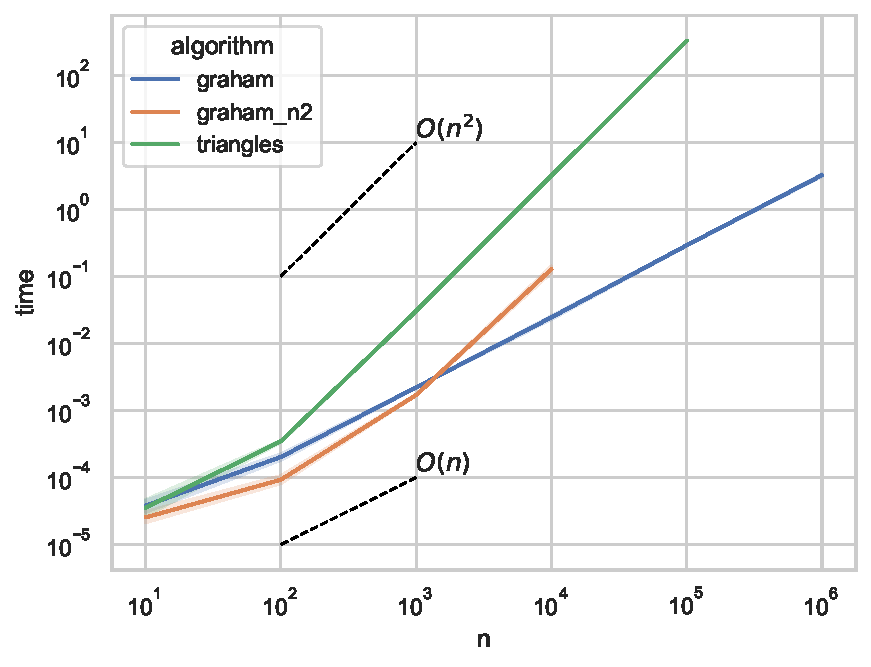
\includegraphics[width=0.7\textwidth]{./figs/time.pdf}
    \end{figure}
\end{frame}

\begin{frame}{Caminho do Baricentro para exterior}

  \begin{columns}
    \begin{column}{0.5\textwidth}
      \begin{itemize}
        \item Encontrar o triângulo que contém o baricentro
        \item Adicionar o triângulo em pilha
        \item Enquanto topo da pilha não é triângulo com lado para exterior:
        \begin{itemize}
          \item Marcar topo da pilha como visitado
          \item Empilhar vizinho não visitado.
          \item Caso não exista, desempilha.
        \end{itemize}
      \end{itemize}
    \end{column}
    \begin{column}{0.5\textwidth}
      \begin{figure}
        \begin{overprint}
          \onslide<2>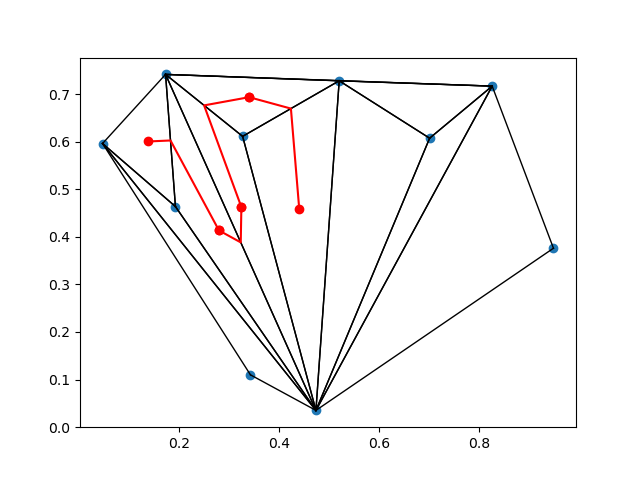
\includegraphics[width=0.95\textwidth]{./figs/bom_exemplo_0_graham_path.png}
          \onslide<3>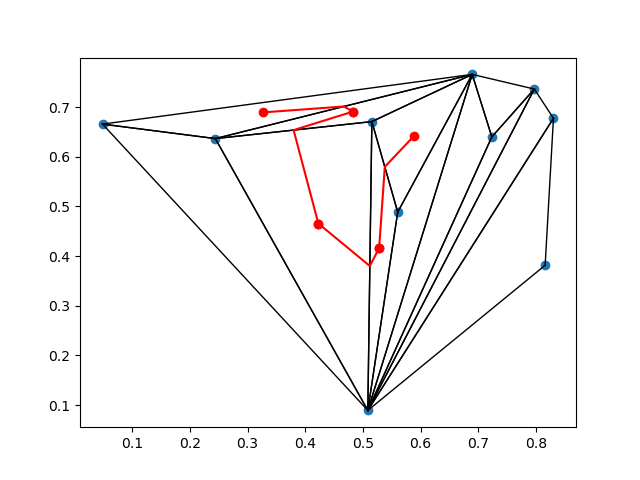
\includegraphics[width=0.95\textwidth]{./figs/bom_exemplo_1_graham_path.png}
          \onslide<4>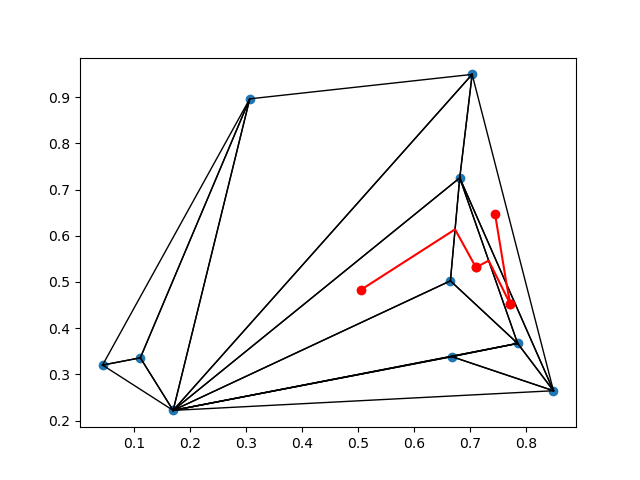
\includegraphics[width=0.95\textwidth]{./figs/bom_exemplo_2_graham_path.png}
        \end{overprint}
      \end{figure}
    \end{column}
  \end{columns}
  
\end{frame}

\end{document}
